\section{实验与结果分析}

\subsubsection{实验设置与对比方法}

所有实验均在基于Ubuntu 20.04操作系统的Kaggle Notebook环境完成,硬件配置采用Kaggle提供的单张NVIDIA P100 GPU(16GB显存)和13GB RAM内存,软件环境基于PyTorch 1.12.0框架,搭配CUDA 11.3加速库。

所有实验共100轮训练,使用初始学习率为$ 1 \times 10^{-4} $Adam优化器,网络权重的初始化采用He normal。同时,每轮训练结束后在验证集上评估,保存Dice得分最高的模型权重。

本文在进行模型评估时,以Dice系数作为核心评价指标,用于衡量模模型在分割任务中预测结果与真实标签之间的重叠程度,是医学图像分割中最常用且最敏感的评估指标之一。为了更全面地反映模型性能,辅以Jaccard指数、F1分数、准确率(Accuracy)、精确率(Precision)与召回率(Recall)等多维度指标进行综合评估。

\subsection{消融实验}

为系统评估各改进模块对模型语义分割性能的影响,本研究设计了一系列消融实验,围绕模型结构、损失函数与训练策略三个层面展开。以基准U-Net模型作为对照组,逐步引入或移除关键组件,包括跳跃连接、注意力机制、数据增强策略、以及不同的损失函数组合,来观察每项设计对模型性能的独立贡献与协同增益。

所有消融实验均基于ISIC 2018皮肤癌图像分割数据集进行,采用 8:2 比例划分训练集与验证集,并在固定的模型训练框架和超参数设置下进行公平比较。通过精心设计的分组实验与逐项对照分析,本节将展示各模块在模型收敛速度、最终性能、错误类型等方面的具体影响,为构建最终优化方案提供理论依据与实证支撑。

\subsubsection{基准模型性能验证}

在消融实验中,基准U-Net模型使用原始U-Net网络结构,配合混合损失函数和Adam优化器进行训练,关于损失函数和优化器的具体参数设置已在第三章阐述。此外,基准模型的训练未采用任何形式的数据增强或正则化操作,以便纯粹评估其建模能力与收敛特性。

为全面评估基准 U-Net 模型在验证集上的性能表现,图~\ref{fig:base_unet_metrics} 展示了训练过程中多个关键评估指标(包括 Dice 系数、Jaccard 指数、Accuracy、Precision、Recall、F1-Score、Specificity 及 Loss)随 epoch 变化的趋势曲线。训练曲线反映了模型收敛过程及其在训练与验证集上的性能差异,可用于分析模型的拟合能力与泛化效果。

\begin{figure}[!htbp]
    \centering
    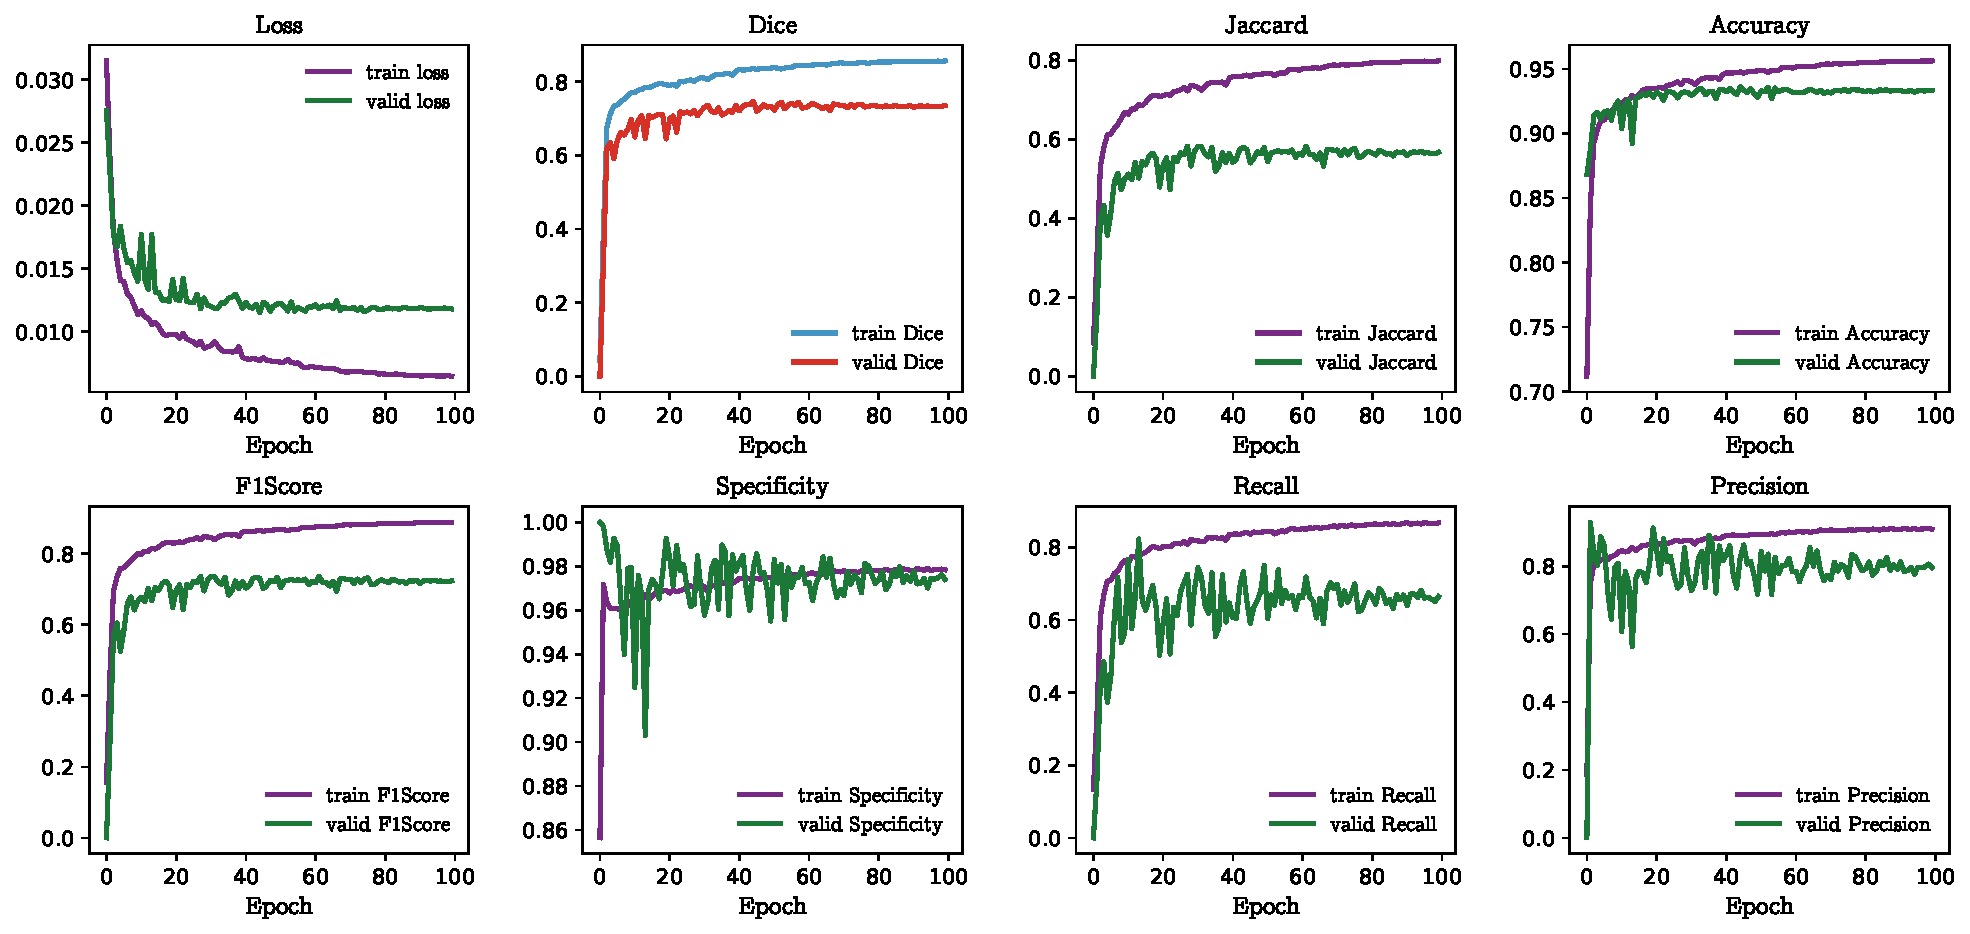
\includegraphics[width=\textwidth]{fig/base_unet_metrics.pdf}
    \caption{基准U-Net模型训练过程中的性能指标变化趋势}
    \label{fig:base_unet_metrics}
\end{figure}

同时,为便于后续实验中基于最优状态进行比较,本研究以验证集 Dice 指标达到最大值的 epoch 作为标准,提取该时刻对应的各项指标结果并作为基准性能对比点,相关数值如表。

\begin{table}[htbp]
    \centering
    \caption{基线U-Net模型在验证集Dice达到最优时(第13轮)的各项性能指标}
    \label{tab:baseline_metrics_horizontal}
    \begin{tabular}{ccccccccc}
        \toprule
        指标 & Dice & F1-score & Jaccard & Precision & Recall & Accuracy & Specificity & Val-Loss \\
        \midrule
        指标值 0.7077 & 0.7030 & 0.5420 & 0.7856 & 0.6266 & 0.9264 & 0.9667 & 0.01312 \\
        \bottomrule
    \end{tabular}
\end{table}

\subsubsection{消融实验结果及分析}


\subsection{泛化性测试}
%在不同医学图像模态(如CT、MRI)和不同器官分割任务中测试改进方法的泛化能力。
%分析模型在不同任务中的表现,验证其在多种场景下的适用性和鲁棒性。


\subsection{方法局限性讨论}
%研究在不同大小的训练数据集下,改进方法的模型性能变化。
%分析模型在小数据集和大数据集上的表现差异,评估其对数据量的敏感性和鲁棒性。
